\documentclass[class=NCU_thesis, crop=false]{standalone}
\begin{document}

\chapter{研究方法}
本章節中,
將闡述本文所開發之嬰兒危險監測系統,
與其兩項核心辨識功能,
透過以下四章子節進行說明:
嬰兒危險監測系統、臉部遮擋辨識、姿勢辨識及危險情境判斷方法。

\section{嬰兒危險監測系統}
本研究針對嬰兒影像畫面進行偵測,
判斷其臉部遮擋與否或姿勢是否不當,
而處於危險情境中。

\subsection{系統流程}
本系統之完整流程如\cref{fig:fig-flow-chart-system}所示:
首先,
讀取一段待觀測之嬰兒影片,
將影片切成影像以進行後續危險偵測。
針對每幀嬰兒畫面,
系統對其臉部遮擋及姿勢進行辨識,
分別輸出模型判斷之結果。
接著,
若分析嬰兒為警示狀態,
則進行危險情境判斷,
以決定系統是否發出警示。
最後,
檢查所觀測之影片結束與否,
若尚未結束,
則同前述步驟接續進行偵測。
\fig[1][fig:fig-flow-chart-system][!hbt]{fig-flow-chart-system.png}[系統流程圖][系統流程圖]

而系統包含之兩項辨識功能及危險情境判斷,
將分別於\ref{sec:chapter_method_face}節、\ref{sec:chapter_method_posture}節及\ref{sec:chapter_method_danger}節進行詳細的介紹。

% (1) 嬰兒臉部遮擋辨識:
% 先將嬰兒影像擷取出臉部畫面,
% 再透過此模型判斷其臉部是否遭非奶嘴之異物遮蔽,
% 若是,則嬰兒為警示狀態;
% (2) 嬰兒危險動作辨識:
% 將拍攝之嬰兒全身影像透過此模型進行辨識,
% 判斷嬰兒為正躺或坐姿之安全狀態,
% 或為需警示的趴躺及站立姿勢。
% 若兩模型結果皆為安全,
% 則系統會判斷嬰兒狀態為安全,
% 否則,嬰兒狀態則為警示。
% 此二部分之詳細方法,
% 將於3.2節及3.3節進行介紹。

\subsection{使用場域}
本研究中,
目前僅針對單一嬰兒之情境進行辨識。
而系統所讀取的影片可為俯視、平視等不同視角之畫面,
不限定需架設於嬰兒床上方或房間某處,
故當嬰兒在較大空間之環境活動時,
可同時透過不同視角進行危險監測。
另外,
建議嬰兒佔據畫面比例一半以上,
且穿著之服飾及背景環境顏色與膚色相異度較大,
則能有較佳的辨識結果。

\section{臉部遮擋辨識}
\label{sec:chapter_method_face}
如前言所述,
目前醫界對於嬰兒猝死症之相關因素研究指出,
注意嬰兒臉部是否遭遮蔽,
將有助於降低此症的發生;
另亦有研究發現嬰兒使用奶嘴,
對於預防嬰兒猝死症有幫助。
因此,
嬰兒使用奶嘴之情境,
將不列入本文對於臉部遮擋的定義。

起初,
基於電腦視覺及影像處理技術,
例如:利用Cb, Cr色彩空間及ellipse clustering
~\cite{tang_hands_2008, li_face_2011, noauthor_python_nodate, walkonnet_python_nodate}
等偵測膚色,
判斷嬰兒臉部是否出現非膚色之區塊,
以進行臉部遮擋辨識,
其效果如\cref{fig:fig-skin-detection}。
\fig[0.7][fig:fig-skin-detection][!hbt]{fig-skin-detection.png}[臉部膚色偵測][臉部膚色偵測]

而後考量能有較佳的推廣性,
因此,
本研究改為使用深度學習技術進行臉部遮擋辨識,
針對嬰兒面部影像自製資料集,
以訓練可辨識三種嬰兒臉部狀態之模型。
而資料集之詳細內容將於\ref{sec:chapter_method_face_dataset}節進行介紹。

本部分之流程如\cref{fig:fig-flow-chart-face}:
首先,
讀取嬰兒影像,
並透過SSD演算法~\cite{ye_face_2021}偵測臉部,
若未找到面部,
則再以RetinaFace演算法~\cite{deng_retinaface_2020}偵測之,
若仍未能找到嬰兒臉部,
則輸出「無臉」之結果;
接著,
將透過人臉偵測演算法擷取出之臉部畫面,
使用本文訓練的臉部遮擋模型辨識面部遮蔽情形,
並輸出判斷結果;
若輸出為「安全」或「奶嘴」,
此部分判斷嬰兒為安全狀態,
而若結果為「警示」,
則分析嬰兒為警示狀態。
\fig[1][fig:fig-flow-chart-face][!hbt]{fig-flow-chart-face.png}[臉部遮擋辨識流程圖][臉部遮擋辨識流程圖]

\subsection{臉部偵測}
由於本研究中之臉部遮擋辨識僅需關注嬰兒臉部畫面,
故本文會先透過人臉偵測演算法進行前處理,
以獲得只涵蓋嬰兒面部範圍之影像。
經多方實驗現有人臉偵測演算法後,
同時考量嬰兒臉部偵測之正確率及執行時間,
最終本研究選用SSD及RetinaFace等演算法進行人臉偵測,
其效果如\cref{fig:fig-face-detection}。
\begin{figure}[!hbt]
    \centering
    \subcaptionbox
        {原始影像
        \label{fig:fig-face-detection-original}}
        {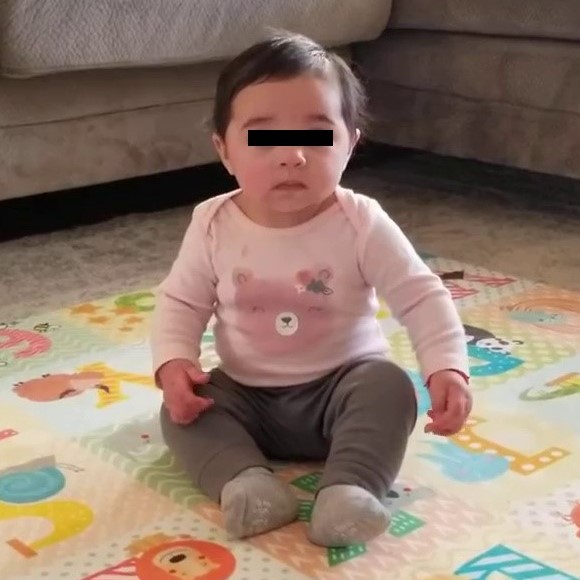
\includegraphics[width=0.3\linewidth]{fig-face-detection-original}}
    ~
    \subcaptionbox
        {使用RetinaFace~\cite{deng_retinaface_2020}
        \label{fig:fig-face-detection-retinaface}}
        {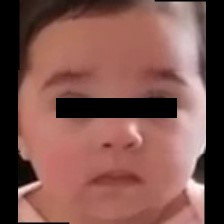
\includegraphics[width=0.3\linewidth]{fig-face-detection-retinaface}}
    ~
    \subcaptionbox
        {使用SSD~\cite{ye_face_2021}
        \label{fig:fig-face-detection-ssd}}
        {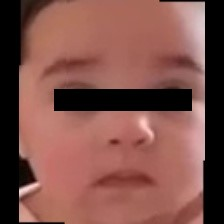
\includegraphics[width=0.3\linewidth]{fig-face-detection-ssd}}
    \caption{嬰兒臉部偵測結果}
    \label{fig:fig-face-detection}
\end{figure}

\subsection{嬰兒臉部資料集}
\label{sec:chapter_method_face_dataset}
由於目前未有公開之嬰兒資料集,
故本論文使用之嬰兒影像,
皆收集自網路上真實嬰兒的彩色照片或影片,
再經前處理及分類標示而成。

本部分資料集將嬰兒臉部狀態分為三類,
分別為臉部無遮蔽、臉部遮蔽物為奶嘴及臉部遮蔽物非奶嘴,
各類別含1197張、1146張及1132張,
總共3475張影像。
而三類詳細定義如下:
\begin{enumerate}
    \item 臉部無遮蔽:嬰兒五官皆未被遮擋,為安全狀態,如\cref{fig:fig-face-uncovered}。
    \item 臉部遮蔽物為奶嘴:嬰兒正在使用奶嘴,為安全狀態,如\cref{fig:fig-face-covered-by-pacifier}。
    \item 臉部遮蔽物非奶嘴:嬰兒臉部因溢奶遭嘔吐物遮蔽,或被毛巾等其他外物遮蓋,而可能造成窒息危險,為警示狀態,如\cref{fig:fig-face-covered-by-foreign-matter}。
\end{enumerate}
\begin{figure}[!hbt]
    \centering
    \subcaptionbox
        {臉部無遮蔽
        \label{fig:fig-face-uncovered}}
        {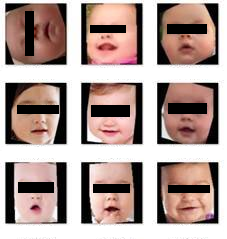
\includegraphics[width=0.45\linewidth]{fig-face-uncovered}}
    ~
    \subcaptionbox
        {臉部遮蔽物為奶嘴
        \label{fig:fig-face-covered-by-pacifier}}
        {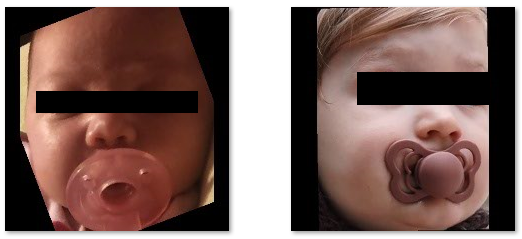
\includegraphics[width=0.45\linewidth]{fig-face-covered-by-pacifier}}
    ~
    \subcaptionbox
        {臉部遭異物遮擋
        \label{fig:fig-face-covered-by-foreign-matter}}
        {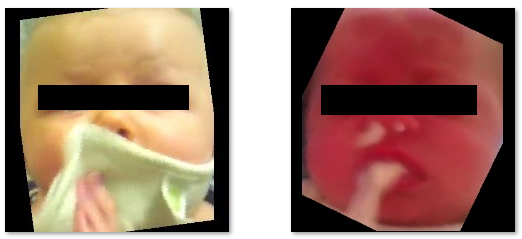
\includegraphics[width=0.45\linewidth]{fig-face-covered-by-foreign-matter}}
    \caption{嬰兒臉部資料集}
    \label{fig:fig-face-dataset}
\end{figure}

並將完整資料集分成訓練、測試及驗證集,
各部分占比為70\%、20\%及10\%,
即各有2436張、697張及342張影像。

\subsection{模型訓練}
本論文使用\ref{sec:chapter_method_face_dataset}節之嬰兒臉部資料集,
以ResNet50~\cite{he_deep_2016}進行臉部遮擋辨識模型之訓練,
最終達成辨識三種嬰兒臉部狀態:安全、使用奶嘴及警示。

\section{姿勢辨識}
\label{sec:chapter_method_posture}
承前言所述,
除了臉部遮蔽可能造成嬰兒猝死症外,
嬰兒做出不適當的姿勢或動作也常為意外發生原因,
例如:嬰兒側躺或趴睡時,
因頸部肌肉較弱等原因,
無力自行將臉移開,
造成呼吸困難而窒息死亡;
或者當嬰兒自行站立,
而有可能爬落嬰兒床等,
亦可能使嬰兒處於危險情境中。

起初,
本文使用OpenPose~\cite{cao_openpose_2019}及MediaPipe Pose~\cite{noauthor_pose_nodate}等演算法,
進行嬰兒骨架之偵測,
結果如\cref{fig:fig-posture-skeleton-detection}及\cref{fig:fig-posture-skeleton-detection-2};
且由\cref{fig:fig-posture-skeleton-detection-viewport}可看出,
嬰兒骨架圖在俯視角與平視角中多有相似之處,
若欲達到從非限定視角辨識嬰兒動作之目標,
則無法僅透過骨架圖進行辨識。
\begin{figure}[!hbt]
    \centering
    \subcaptionbox
        {原始影像
        \label{fig:fig-posture-skeleton-detection-original}}
        {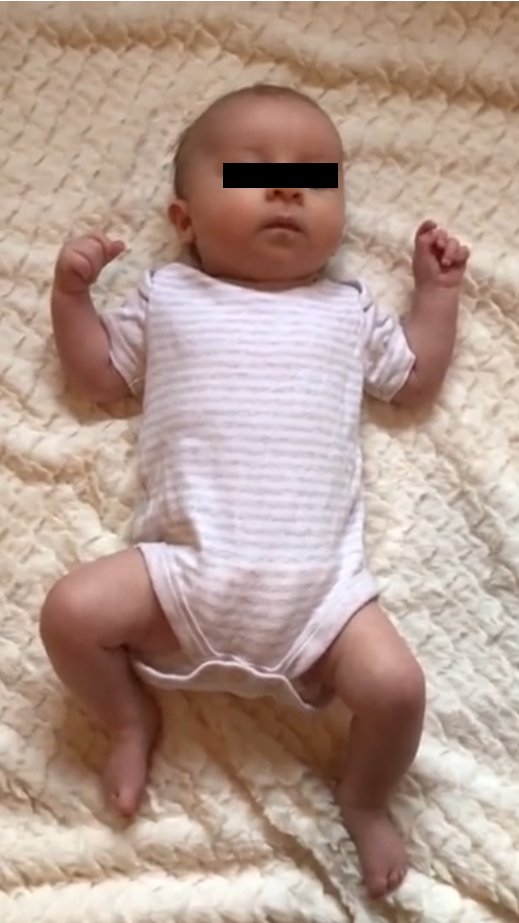
\includegraphics[width=0.3\linewidth]{fig-posture-skeleton-detection-original}}
    ~
    \subcaptionbox
        {使用OpenPose~\cite{cao_openpose_2019}
        \label{fig:fig-posture-skeleton-detection-openpose}}
        {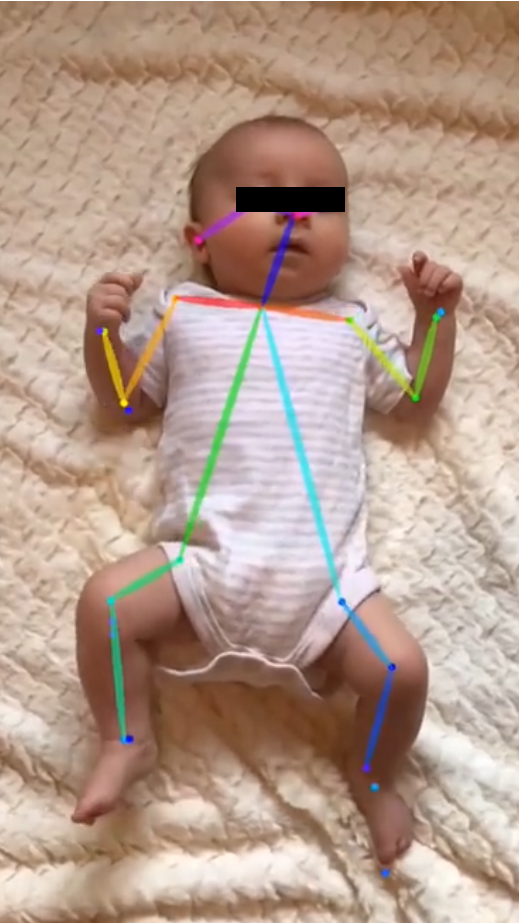
\includegraphics[width=0.3\linewidth]{fig-posture-skeleton-detection-openpose}}
    ~
    \subcaptionbox
        {使用MediaPipe Pose~\cite{noauthor_pose_nodate}
        \label{fig:fig-posture-skeleton-detection-mediapipe}}
        {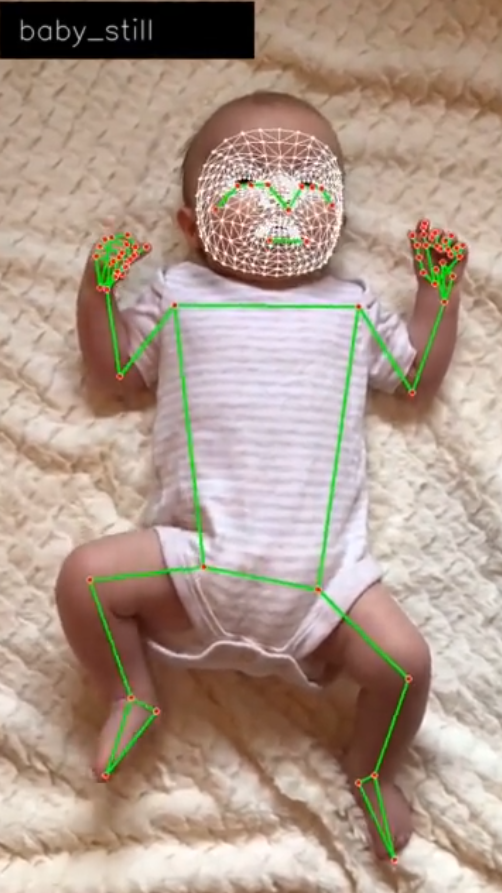
\includegraphics[width=0.3\linewidth]{fig-posture-skeleton-detection-mediapipe}}
    \caption{嬰兒正躺之骨架偵測結果}
    \label{fig:fig-posture-skeleton-detection}
\end{figure}
\begin{figure}[!hbt]
    \centering
    \subcaptionbox
        {原始影像
        \label{fig:fig-posture-skeleton-detection-2-original}}
        {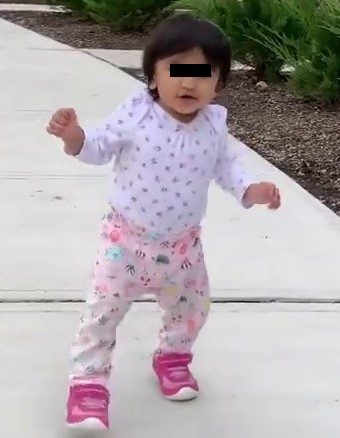
\includegraphics[width=0.3\linewidth]{fig-posture-skeleton-detection-2-original}}
    ~
    \subcaptionbox
        {使用OpenPose~\cite{cao_openpose_2019}
        \label{fig:fig-posture-skeleton-detection-2-openpose}}
        {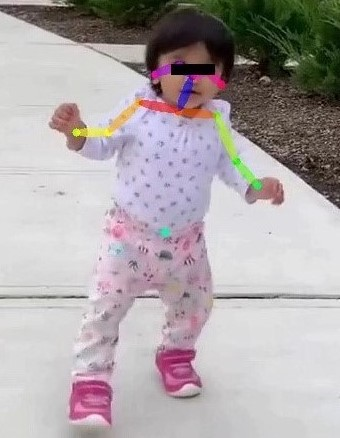
\includegraphics[width=0.3\linewidth]{fig-posture-skeleton-detection-2-openpose}}
    ~
    \subcaptionbox
        {使用MediaPipe Pose~\cite{noauthor_pose_nodate}
        \label{fig:fig-posture-skeleton-detection-2-mediapipe}}
        {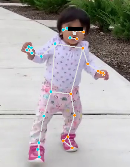
\includegraphics[width=0.3\linewidth]{fig-posture-skeleton-detection-2-mediapipe}}
    \caption{嬰兒站姿之骨架偵測結果}
    \label{fig:fig-posture-skeleton-detection-2}
\end{figure}
\begin{figure}[!hbt]
    \centering
    \subcaptionbox
        {俯視嬰兒躺姿
        \label{fig:fig-posture-skeleton-detection-viewport-lying}}
        {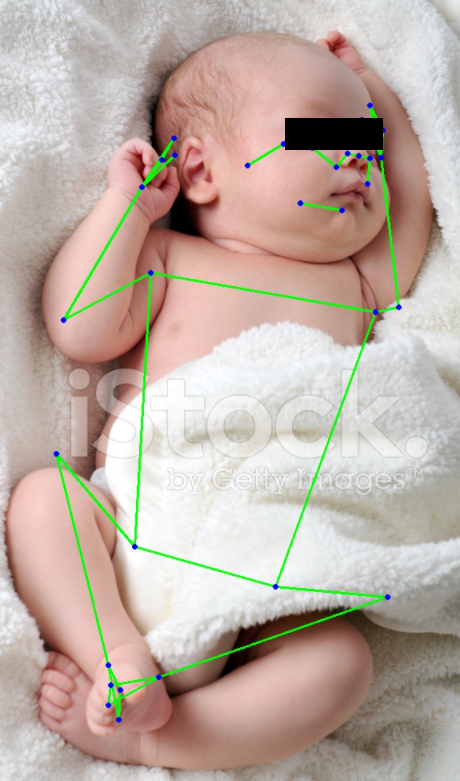
\includegraphics[width=0.3\linewidth]{fig-posture-skeleton-detection-viewport-lying}}
    ~
    \subcaptionbox
        {平視嬰兒坐姿
        \label{fig:fig-posture-skeleton-detection-viewport-sit}}
        {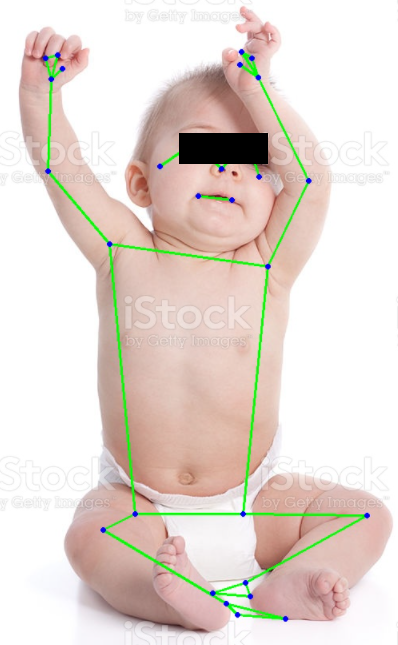
\includegraphics[width=0.3\linewidth]{fig-posture-skeleton-detection-viewport-sit}}
    \caption{不同視角之嬰兒骨架偵測結果}
    \label{fig:fig-posture-skeleton-detection-viewport}
\end{figure}

因此,
本研究改為基於深度學習技術進行嬰兒動作辨識,
使用自行收集之嬰兒影像資料集,
訓練可辨識四種嬰兒基礎姿勢之模型。
而資料集之詳細內容將於\ref{sec:chapter_method_posture_dataset}節進行介紹。

本部分流程如\cref{fig:fig-flow-chart-posture}:
讀取嬰兒影像後,
使用本文訓練的姿勢模型辨識嬰兒動作,
並輸出判斷結果;
若輸出為「正躺」或「坐姿」,
此部分判斷嬰兒為安全狀態,
而若結果為「趴躺」或「站立」,
則分析嬰兒為警示狀態。
\fig[1][fig:fig-flow-chart-posture][!hbt]{fig-flow-chart-posture.png}[姿勢辨識流程圖][姿勢辨識流程圖]

\subsection{嬰兒姿勢資料集}
\label{sec:chapter_method_posture_dataset}
由於目前未有公開之嬰兒資料集,
故本論文使用之嬰兒影像,
皆收集自網路上真實嬰兒的彩色照片或影片,
再經前處理及分類標示而成。

起初,
本研究將嬰兒姿勢分為五類:正躺、趴睡、爬行、坐姿及站立,
而趴睡及爬行二類時常發生互相誤判,
致使辨識錯誤率高。
推測原因為此二類嬰兒皆呈現腹面朝下之姿,
不同處在於四肢及軀體是否貼地,
如\cref{fig:fig-posture-sleep-on-stomack-detail}所示,
但若接續細分姿勢,
將使分類過細。
\begin{figure}[!hbt]
    \centering
    \subcaptionbox
        {四肢及軀體皆貼地
        \label{fig:fig-posture-sleep-on-stomack-detail-1}}
        {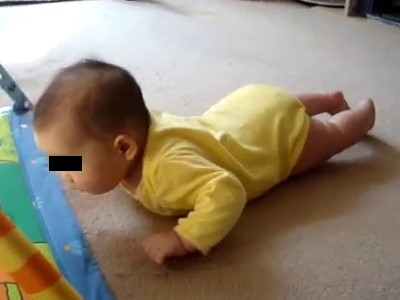
\includegraphics[width=0.3\linewidth]{fig-posture-sleep-on-stomack-detail-1}}
    ~
    \subcaptionbox
        {僅手掌與小腿貼地
        \label{fig:fig-posture-sleep-on-stomack-detail-2}}
        {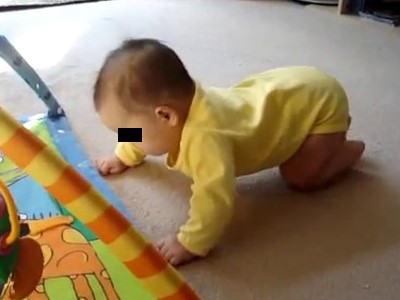
\includegraphics[width=0.3\linewidth]{fig-posture-sleep-on-stomack-detail-2}}
    ~
    \subcaptionbox
        {僅手掌與腳掌貼地
        \label{fig:fig-posture-sleep-on-stomack-detail-3}}
        {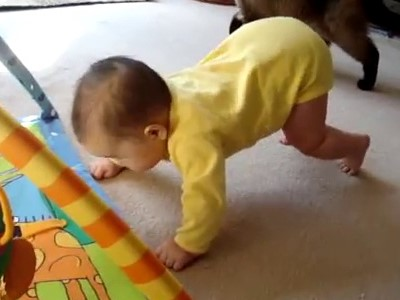
\includegraphics[width=0.3\linewidth]{fig-posture-sleep-on-stomack-detail-3}}
    \caption{嬰兒腹面朝下之姿}
    \label{fig:fig-posture-sleep-on-stomack-detail}
\end{figure}

因此,
最終本部分資料集將嬰兒姿勢分成基礎四類,
包含正躺(腹面朝上)、趴躺(腹面朝下)、坐姿及站立,
各類別含3774張、3921張、3900張及3821張,
總共15416張照片。
且為了能有較廣泛的使用情境,
所收集之嬰兒影像不限定拍攝視角,
包含俯視及平視等。
而對於此四類姿勢之詳細定義如下:
\begin{enumerate}
    \item 正躺:嬰兒腹部面朝上,背部貼於水平面,而頭部及四肢位置不限,如\cref{fig:fig-posture-sleep-on-back}。
    \item 趴躺:嬰兒腹部面朝下,包含趴睡及爬行等多動作,而頭部及四肢位置不限,如\cref{fig:fig-posture-sleep-on-stomach}。
    \item 坐姿:嬰兒臀部貼於水平面,且背部未貼於同一平面,而頭部及四肢位置不限,如\cref{fig:fig-posture-sit}。
    \item 站立:嬰兒腳掌貼於水平面,且腹部和背部皆未平行於此水平面,而頭部及上肢位置不限,如\cref{fig:fig-posture-stand}。
\end{enumerate}
\begin{figure}[!hbt]
    \centering
    \subcaptionbox
        {正躺
        \label{fig:fig-posture-sleep-on-back}}
        {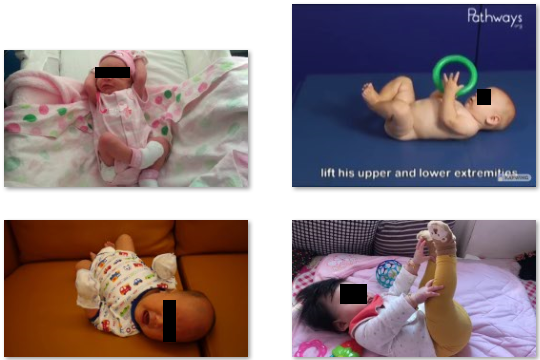
\includegraphics[width=0.45\linewidth]{fig-posture-sleep-on-back}}
    ~
    \subcaptionbox
        {趴躺
        \label{fig:fig-posture-sleep-on-stomach}}
        {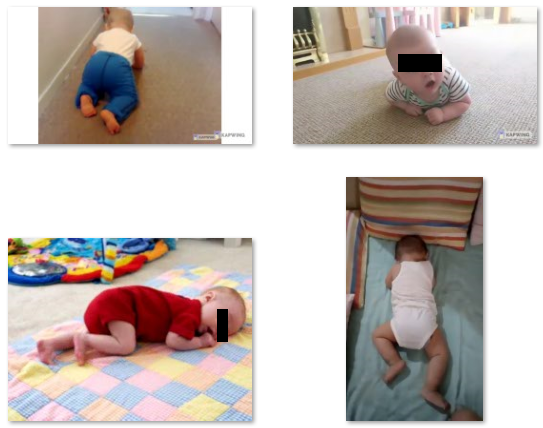
\includegraphics[width=0.45\linewidth]{fig-posture-sleep-on-stomach}}
    ~
    \subcaptionbox
        {坐姿
        \label{fig:fig-posture-sit}}
        {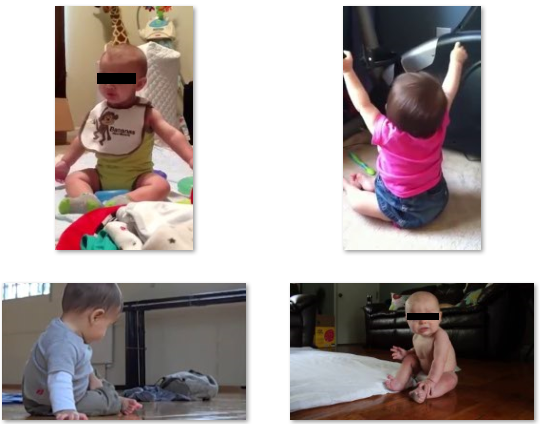
\includegraphics[width=0.45\linewidth]{fig-posture-sit}}
    ~
    \subcaptionbox
        {站立
        \label{fig:fig-posture-stand}}
        {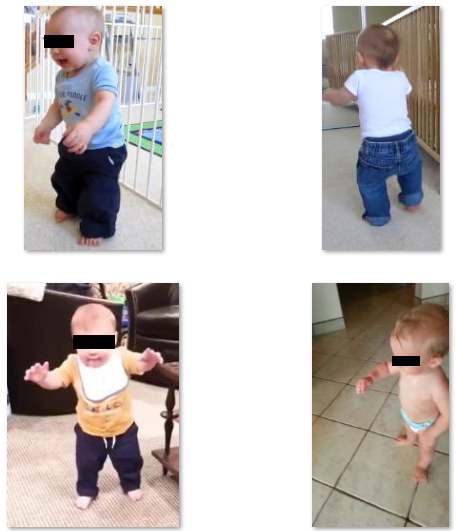
\includegraphics[width=0.45\linewidth]{fig-posture-stand}}
    \caption{嬰兒姿勢資料集}
    \label{fig:fig-face-dataset}
\end{figure}

並將完整資料集分成訓練、測試及驗證集,
各部分占比為70\%、25\%及5\%,
即各有10815張、3857張及744張影像。

\subsection{模型訓練}
本論文使用\ref{sec:chapter_method_posture_dataset}節之嬰兒姿勢資料集,
以ResNet50~\cite{he_deep_2016}進行姿勢辨識模型之訓練,
最終達成辨識四種嬰兒姿勢:正躺、趴躺、坐姿及站立。

\section{危險情境判斷}
\label{sec:chapter_method_danger}
在實際情境中,
當嬰兒做出具危險性之行為時,
需持續一段時間才會導致危險發生,
並不須判斷一幀畫面為警示狀態,
就立即通知照護者。

因此,
本系統使用一變數累積模型判斷嬰兒狀態為警示之幀數,
當此變數超過設定閥值時,
系統才會發出警示提醒照護者。
本部分之流程圖,
請見\cref{fig:fig-flow-chart-danger}。
此步驟不但更符合實際使用情境,
同時亦可減少因模型辨識錯誤而誤判及誤發警報的情形。
\fig[1][fig:fig-flow-chart-danger][!hbt]{fig-flow-chart-danger.png}[危險情境判斷流程圖][危險情境判斷流程圖]

\end{document}